\chapter{Quantile regression}
\label{chap:quantreg}

\section{Introduction}
\label{sec:rq-intro}

In Ordinary Least Squares (OLS) regression, the fitted values,
$\hat{y}_i = X_i\hat{\beta}$, represent the \emph{conditional mean} of
the dependent variable --- conditional, that is, on the regression
function and the values of the independent variables.  In median
regression, by contrast and as the name implies, fitted values
represent the \emph{conditional median} of the dependent variable.  It
turns out that the principle of estimation for median regression is
easily stated (though not so easily computed), namely, choose
$\hat{\beta}$ so as to minimize the sum of absolute residuals.  Hence
the method is known as Least Absolute Deviations or LAD.  While the OLS
problem has a straightforward analytical solution, LAD is a linear
programming problem.

Quantile regression is a generalization of median regression: the
regression function predicts the conditional $\tau$-quantile of the
dependent variable --- for example the first quartile ($\tau = .25$)
or the ninth decile ($\tau = .90$).

If the classical conditions for the validity of OLS are satisfied ---
that is, if the error term is independently and identically
distributed, conditional on $X$ --- then quantile regression is
redundant: all the conditional quantiles of the dependent variable
will march in lockstep with the conditional mean.  Conversely, if
quantile regression reveals that the conditional quantiles behave in a
manner quite distinct from the conditional mean, this suggests that
OLS estimation is problematic.

As of version 1.7.5, \app{gretl} offers quantile regression
functionality (in addition to basic LAD regression, which has been
available since early in \app{gretl}'s history via the \texttt{lad}
command).\footnote{We gratefully acknowledge our borrowing from the
  \texttt{quantreg} package for GNU \textsf{R} (version 4.17).  The
  core of the \texttt{quantreg} package is composed of Fortran code
  written by Roger Koenker; this is accompanied by various driver and
  auxiliary functions written in the \textsf{R} language by Koenker
  amd Martin M\"achler.  The latter functions have been re-worked in C
  for \app{gretl}.  We have added some guards against potential
  numerical problems in small samples.}

\section{Basic syntax}

The basic invocation of quantile regression is

\vspace{1em}
\noindent
\qquad \texttt{quantreg} \textsl{tau} \textsl{reglist}
\vspace{1em}

where

\begin{itemize}
\item \textsl{reglist} is a standard \textsf{gretl} regression list
  (dependent variable followed by regressors, including the constant
  if an intercept is wanted); and
\item \textsl{tau} is the desired conditional quantile, in the range
  0.01 to 0.99, given either as a numerical value or the name of a
  pre-defined scalar variable (but see below for a further option).
\end{itemize}

Estimation is via the Frisch--Newton interior point solver (Portnoy
and Koenker, 1997), which is substantially faster than the
``traditional'' Barrodale--Roberts (1974) simplex approach for large
problems.

By default, standard errors are computed according to the asymptotic
formula given by Koenker and Bassett (1978).  Alternatively, if the
\verb|--robust| option is given, we use the sandwich estimator
developed in Koenker and Zhao (1994).\footnote{These correspond to the
  \texttt{iid} and \texttt{nid} options in \textsf{R}'s
  \texttt{quantreg} package, respectively.}

\section{Confidence intervals}

An option \verb|--intervals| is available.  When this is given we
print confidence intervals for the parameter estimates instead of
standard errors.  These intervals are computed using the rank
inversion method and in general they are asymmetrical about the point
estimates --- that is, they are not simply ``plus or minus so many
standard errors''.  The specifics of the calculation are inflected by
the \verb|--robust| option: without this, the intervals are computed
on the assumption of IID errors (Koenker, 1994); with it, they use the
heteroskedasticity-robust estimator developed by Koenker and Machado
(1999).

By default, 90 percent intervals are produced.  You can change this by
appending a confidence value (expressed as a decimal fraction) to the
intervals option, as in

\vspace{1em}
\noindent
\qquad \texttt{quantreg} \textsl{tau} \textsl{reglist} \verb|--intervals=.95|
\vspace{1em}

When the confidence intervals option is selected, the parameter
estimates are calculated using the Barrodale--Roberts method.  This is
simply because the Frisch--Newton code does not currently support the
calculation of confidence intervals.

Two further details.  First, the mechanisms for generating confidence
intervals for quantile estimates require that the model has at least
two regressors (including the constant).  If the \verb|--intervals|
option is given for a model containing only one regressor, an error is
flagged.  Second, when a model is estimated in this mode, you can
retrieve the confidence intervals using the accessor \verb|$coeff_ci|.
This produces a $k \times 2$ matrix, where $k$ is the number of
regressors.  The lower bounds are in the first column, the upper
bounds in the second.

\section{Multiple quantiles}

As a further option, you can give \textsl{tau} as a matrix --- either
the name of a predefined matrix or in numerical form, as in
\verb+{.05, .25, .5, .75, .95}+.  This implies the \verb|--intervals|
option.  The given model is estimated for all the $\tau$ values and
the results are printed in a special form:

{\small
\begin{verbatim}
Model 1: Quantile estimates using the 235 observations 1-235
Dependent variable: foodexp
With 90 percent confidence intervals

      VARIABLE      TAU    COEFFICIENT      LOWER        UPPER

  const             0.05      124.880      98.3021      130.517
                    0.25      95.4835      73.7861      120.098
                    0.50      81.4822      53.2592      114.012
                    0.75      62.3966      32.7449      107.314
                    0.95      64.1040      46.2649      83.5790

  income            0.05     0.343361     0.343327     0.389750
                    0.25     0.474103     0.420330     0.494329
                    0.50     0.560181     0.487022     0.601989
                    0.75     0.644014     0.580155     0.690413
                    0.95     0.709069     0.673900     0.734441
\end{verbatim}
}

The \app{gretl} GUI has an entry for Quantile Regression (under
\textsf{/Model/Robust estimation}), and you can select multiple
quantiles there too.  In that context, just give space-separated
numerical values (as per the predefined options, shown in a drop-down
list).  

When you estimate a model in this way most of the standard menu items
in the model window are disabled, but one extra item is available ---
graphs showing the $\tau$ sequence for a given coefficient in
comparison with the OLS coefficient.  An example is shown in
Figure~\ref{fig:tau}.  This sort of graph provides a simple means of
judging whether quantile regression is redundant (OLS is fine) or
informative.  

In the example shown --- based on data on household income and food
expenditure gathered by Ernst Engel (1821--1896) --- it seems clear
that simple OLS regression is potentially misleading.  The
``crossing'' of the OLS estimate by the quantile estimates is very
marked.  

\begin{figure}
  \centering
  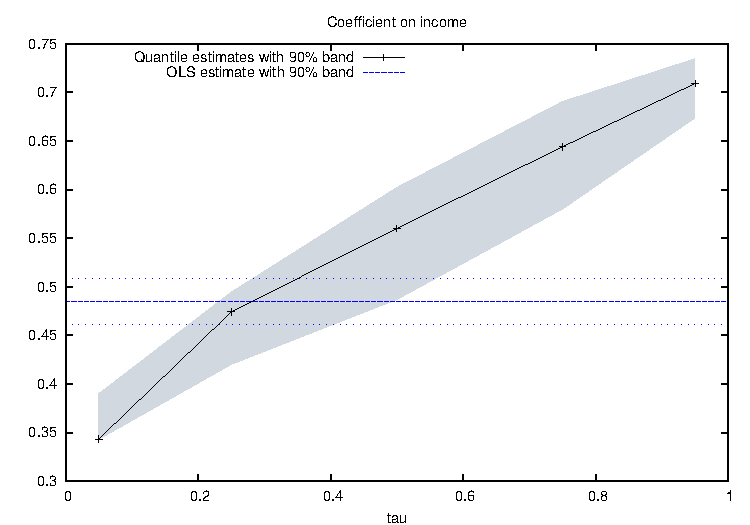
\includegraphics{figures/tau-sequence}
  \caption{The coefficient on income, dependent variable is
    expenditure on food; Ernst Engel's data}
  \label{fig:tau}
\end{figure}

However, it is not always clear what implications should be drawn from
this sort of conflict.  With the Engel data there are two issues to
consider.  First, Engel's famous ``law'' claims an income-elasticity
of food consumption that is less than one, and talk of elasticities
suggests a logarithmic formulation of the model.  Second, there are
two apparently anomalous observations in the data set: household 105
has the third-highest income but unexpectedly low expenditure on food
(as judged from a simple scatter plot), while household 138 (which
also has unexpectedly low food consumption) has much the highest
income, almost twice that of the next highest.

With $n = 235$ it seems reasonable to consider dropping these
observations.  If we do so, and adopt a log--log formulation, we get
the plot shown in Figure~\ref{fig:tau2}.  The quantile estimates still
cross the OLS estimate, but the ``evidence against OLS'' is much less
compelling: the 90 percent confidence bands of the respective
estimates overlap at all the quantiles considered.

\begin{figure}
  \centering
  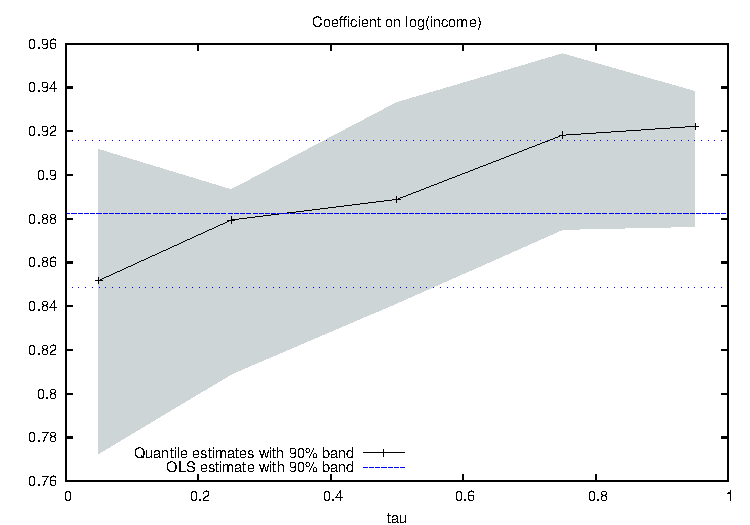
\includegraphics{figures/tau-sequence2}
  \caption{Coefficient on log of income, dependent variable is log of
    expenditure on food; 2 observations dropped from full Engel data
    set.}
  \label{fig:tau2}
\end{figure}






